
\documentclass{article}
\usepackage{graphicx, color}
\IfFileExists{upquote.sty}{\usepackage{upquote}}{}
\definecolor{fgcolor}{rgb}{0.267, 0.267, 0.267}
\newcommand{\hlnumber}[1]{\textcolor[rgb]{0,0,0}{#1}}%
\newcommand{\hlfunctioncall}[1]{\textcolor[rgb]{0.501960784313725,0,0.329411764705882}{\textbf{#1}}}%
\newcommand{\hlstring}[1]{\textcolor[rgb]{0.6,0.6,1}{#1}}%
\newcommand{\hlkeyword}[1]{\textcolor[rgb]{0,0,0}{\textbf{#1}}}%
\newcommand{\hlargument}[1]{\textcolor[rgb]{0.690196078431373,0.250980392156863,0.0196078431372549}{#1}}%
\newcommand{\hlcomment}[1]{\textcolor[rgb]{0.180392156862745,0.6,0.341176470588235}{#1}}%
\newcommand{\hlroxygencomment}[1]{\textcolor[rgb]{0.43921568627451,0.47843137254902,0.701960784313725}{#1}}%
\newcommand{\hlformalargs}[1]{\textcolor[rgb]{0.690196078431373,0.250980392156863,0.0196078431372549}{#1}}%
\newcommand{\hleqformalargs}[1]{\textcolor[rgb]{0.690196078431373,0.250980392156863,0.0196078431372549}{#1}}%
\newcommand{\hlassignement}[1]{\textcolor[rgb]{0,0,0}{\textbf{#1}}}%
\newcommand{\hlpackage}[1]{\textcolor[rgb]{0.588235294117647,0.709803921568627,0.145098039215686}{#1}}%
\newcommand{\hlslot}[1]{\textit{#1}}%
\newcommand{\hlsymbol}[1]{\textcolor[rgb]{0,0,0}{#1}}%
\newcommand{\hlprompt}[1]{\textcolor[rgb]{0.266666666666667,0.266666666666667,0.266666666666667}{#1}}%

\usepackage{color}%
 
\newsavebox{\hlnormalsizeboxclosebrace}%
\newsavebox{\hlnormalsizeboxopenbrace}%
\newsavebox{\hlnormalsizeboxbackslash}%
\newsavebox{\hlnormalsizeboxlessthan}%
\newsavebox{\hlnormalsizeboxgreaterthan}%
\newsavebox{\hlnormalsizeboxdollar}%
\newsavebox{\hlnormalsizeboxunderscore}%
\newsavebox{\hlnormalsizeboxand}%
\newsavebox{\hlnormalsizeboxhash}%
\newsavebox{\hlnormalsizeboxat}%
\newsavebox{\hlnormalsizeboxpercent}% 
\newsavebox{\hlnormalsizeboxhat}%
\newsavebox{\hlnormalsizeboxsinglequote}%
\newsavebox{\hlnormalsizeboxbacktick}%

\setbox\hlnormalsizeboxopenbrace=\hbox{\begin{normalsize}\verb.{.\end{normalsize}}%
\setbox\hlnormalsizeboxclosebrace=\hbox{\begin{normalsize}\verb.}.\end{normalsize}}%
\setbox\hlnormalsizeboxlessthan=\hbox{\begin{normalsize}\verb.<.\end{normalsize}}%
\setbox\hlnormalsizeboxdollar=\hbox{\begin{normalsize}\verb.$.\end{normalsize}}%
\setbox\hlnormalsizeboxunderscore=\hbox{\begin{normalsize}\verb._.\end{normalsize}}%
\setbox\hlnormalsizeboxand=\hbox{\begin{normalsize}\verb.&.\end{normalsize}}%
\setbox\hlnormalsizeboxhash=\hbox{\begin{normalsize}\verb.#.\end{normalsize}}%
\setbox\hlnormalsizeboxat=\hbox{\begin{normalsize}\verb.@.\end{normalsize}}%
\setbox\hlnormalsizeboxbackslash=\hbox{\begin{normalsize}\verb.\.\end{normalsize}}%
\setbox\hlnormalsizeboxgreaterthan=\hbox{\begin{normalsize}\verb.>.\end{normalsize}}%
\setbox\hlnormalsizeboxpercent=\hbox{\begin{normalsize}\verb.%.\end{normalsize}}%
\setbox\hlnormalsizeboxhat=\hbox{\begin{normalsize}\verb.^.\end{normalsize}}%
\setbox\hlnormalsizeboxsinglequote=\hbox{\begin{normalsize}\verb.'.\end{normalsize}}%
\setbox\hlnormalsizeboxbacktick=\hbox{\begin{normalsize}\verb.`.\end{normalsize}}%
\setbox\hlnormalsizeboxhat=\hbox{\begin{normalsize}\verb.^.\end{normalsize}}%



\newsavebox{\hltinyboxclosebrace}%
\newsavebox{\hltinyboxopenbrace}%
\newsavebox{\hltinyboxbackslash}%
\newsavebox{\hltinyboxlessthan}%
\newsavebox{\hltinyboxgreaterthan}%
\newsavebox{\hltinyboxdollar}%
\newsavebox{\hltinyboxunderscore}%
\newsavebox{\hltinyboxand}%
\newsavebox{\hltinyboxhash}%
\newsavebox{\hltinyboxat}%
\newsavebox{\hltinyboxpercent}% 
\newsavebox{\hltinyboxhat}%
\newsavebox{\hltinyboxsinglequote}%
\newsavebox{\hltinyboxbacktick}%

\setbox\hltinyboxopenbrace=\hbox{\begin{tiny}\verb.{.\end{tiny}}%
\setbox\hltinyboxclosebrace=\hbox{\begin{tiny}\verb.}.\end{tiny}}%
\setbox\hltinyboxlessthan=\hbox{\begin{tiny}\verb.<.\end{tiny}}%
\setbox\hltinyboxdollar=\hbox{\begin{tiny}\verb.$.\end{tiny}}%
\setbox\hltinyboxunderscore=\hbox{\begin{tiny}\verb._.\end{tiny}}%
\setbox\hltinyboxand=\hbox{\begin{tiny}\verb.&.\end{tiny}}%
\setbox\hltinyboxhash=\hbox{\begin{tiny}\verb.#.\end{tiny}}%
\setbox\hltinyboxat=\hbox{\begin{tiny}\verb.@.\end{tiny}}%
\setbox\hltinyboxbackslash=\hbox{\begin{tiny}\verb.\.\end{tiny}}%
\setbox\hltinyboxgreaterthan=\hbox{\begin{tiny}\verb.>.\end{tiny}}%
\setbox\hltinyboxpercent=\hbox{\begin{tiny}\verb.%.\end{tiny}}%
\setbox\hltinyboxhat=\hbox{\begin{tiny}\verb.^.\end{tiny}}%
\setbox\hltinyboxsinglequote=\hbox{\begin{tiny}\verb.'.\end{tiny}}%
\setbox\hltinyboxbacktick=\hbox{\begin{tiny}\verb.`.\end{tiny}}%
\setbox\hltinyboxhat=\hbox{\begin{tiny}\verb.^.\end{tiny}}%



\newsavebox{\hlscriptsizeboxclosebrace}%
\newsavebox{\hlscriptsizeboxopenbrace}%
\newsavebox{\hlscriptsizeboxbackslash}%
\newsavebox{\hlscriptsizeboxlessthan}%
\newsavebox{\hlscriptsizeboxgreaterthan}%
\newsavebox{\hlscriptsizeboxdollar}%
\newsavebox{\hlscriptsizeboxunderscore}%
\newsavebox{\hlscriptsizeboxand}%
\newsavebox{\hlscriptsizeboxhash}%
\newsavebox{\hlscriptsizeboxat}%
\newsavebox{\hlscriptsizeboxpercent}% 
\newsavebox{\hlscriptsizeboxhat}%
\newsavebox{\hlscriptsizeboxsinglequote}%
\newsavebox{\hlscriptsizeboxbacktick}%

\setbox\hlscriptsizeboxopenbrace=\hbox{\begin{scriptsize}\verb.{.\end{scriptsize}}%
\setbox\hlscriptsizeboxclosebrace=\hbox{\begin{scriptsize}\verb.}.\end{scriptsize}}%
\setbox\hlscriptsizeboxlessthan=\hbox{\begin{scriptsize}\verb.<.\end{scriptsize}}%
\setbox\hlscriptsizeboxdollar=\hbox{\begin{scriptsize}\verb.$.\end{scriptsize}}%
\setbox\hlscriptsizeboxunderscore=\hbox{\begin{scriptsize}\verb._.\end{scriptsize}}%
\setbox\hlscriptsizeboxand=\hbox{\begin{scriptsize}\verb.&.\end{scriptsize}}%
\setbox\hlscriptsizeboxhash=\hbox{\begin{scriptsize}\verb.#.\end{scriptsize}}%
\setbox\hlscriptsizeboxat=\hbox{\begin{scriptsize}\verb.@.\end{scriptsize}}%
\setbox\hlscriptsizeboxbackslash=\hbox{\begin{scriptsize}\verb.\.\end{scriptsize}}%
\setbox\hlscriptsizeboxgreaterthan=\hbox{\begin{scriptsize}\verb.>.\end{scriptsize}}%
\setbox\hlscriptsizeboxpercent=\hbox{\begin{scriptsize}\verb.%.\end{scriptsize}}%
\setbox\hlscriptsizeboxhat=\hbox{\begin{scriptsize}\verb.^.\end{scriptsize}}%
\setbox\hlscriptsizeboxsinglequote=\hbox{\begin{scriptsize}\verb.'.\end{scriptsize}}%
\setbox\hlscriptsizeboxbacktick=\hbox{\begin{scriptsize}\verb.`.\end{scriptsize}}%
\setbox\hlscriptsizeboxhat=\hbox{\begin{scriptsize}\verb.^.\end{scriptsize}}%



\newsavebox{\hlfootnotesizeboxclosebrace}%
\newsavebox{\hlfootnotesizeboxopenbrace}%
\newsavebox{\hlfootnotesizeboxbackslash}%
\newsavebox{\hlfootnotesizeboxlessthan}%
\newsavebox{\hlfootnotesizeboxgreaterthan}%
\newsavebox{\hlfootnotesizeboxdollar}%
\newsavebox{\hlfootnotesizeboxunderscore}%
\newsavebox{\hlfootnotesizeboxand}%
\newsavebox{\hlfootnotesizeboxhash}%
\newsavebox{\hlfootnotesizeboxat}%
\newsavebox{\hlfootnotesizeboxpercent}% 
\newsavebox{\hlfootnotesizeboxhat}%
\newsavebox{\hlfootnotesizeboxsinglequote}%
\newsavebox{\hlfootnotesizeboxbacktick}%

\setbox\hlfootnotesizeboxopenbrace=\hbox{\begin{footnotesize}\verb.{.\end{footnotesize}}%
\setbox\hlfootnotesizeboxclosebrace=\hbox{\begin{footnotesize}\verb.}.\end{footnotesize}}%
\setbox\hlfootnotesizeboxlessthan=\hbox{\begin{footnotesize}\verb.<.\end{footnotesize}}%
\setbox\hlfootnotesizeboxdollar=\hbox{\begin{footnotesize}\verb.$.\end{footnotesize}}%
\setbox\hlfootnotesizeboxunderscore=\hbox{\begin{footnotesize}\verb._.\end{footnotesize}}%
\setbox\hlfootnotesizeboxand=\hbox{\begin{footnotesize}\verb.&.\end{footnotesize}}%
\setbox\hlfootnotesizeboxhash=\hbox{\begin{footnotesize}\verb.#.\end{footnotesize}}%
\setbox\hlfootnotesizeboxat=\hbox{\begin{footnotesize}\verb.@.\end{footnotesize}}%
\setbox\hlfootnotesizeboxbackslash=\hbox{\begin{footnotesize}\verb.\.\end{footnotesize}}%
\setbox\hlfootnotesizeboxgreaterthan=\hbox{\begin{footnotesize}\verb.>.\end{footnotesize}}%
\setbox\hlfootnotesizeboxpercent=\hbox{\begin{footnotesize}\verb.%.\end{footnotesize}}%
\setbox\hlfootnotesizeboxhat=\hbox{\begin{footnotesize}\verb.^.\end{footnotesize}}%
\setbox\hlfootnotesizeboxsinglequote=\hbox{\begin{footnotesize}\verb.'.\end{footnotesize}}%
\setbox\hlfootnotesizeboxbacktick=\hbox{\begin{footnotesize}\verb.`.\end{footnotesize}}%
\setbox\hlfootnotesizeboxhat=\hbox{\begin{footnotesize}\verb.^.\end{footnotesize}}%



\newsavebox{\hlsmallboxclosebrace}%
\newsavebox{\hlsmallboxopenbrace}%
\newsavebox{\hlsmallboxbackslash}%
\newsavebox{\hlsmallboxlessthan}%
\newsavebox{\hlsmallboxgreaterthan}%
\newsavebox{\hlsmallboxdollar}%
\newsavebox{\hlsmallboxunderscore}%
\newsavebox{\hlsmallboxand}%
\newsavebox{\hlsmallboxhash}%
\newsavebox{\hlsmallboxat}%
\newsavebox{\hlsmallboxpercent}% 
\newsavebox{\hlsmallboxhat}%
\newsavebox{\hlsmallboxsinglequote}%
\newsavebox{\hlsmallboxbacktick}%

\setbox\hlsmallboxopenbrace=\hbox{\begin{small}\verb.{.\end{small}}%
\setbox\hlsmallboxclosebrace=\hbox{\begin{small}\verb.}.\end{small}}%
\setbox\hlsmallboxlessthan=\hbox{\begin{small}\verb.<.\end{small}}%
\setbox\hlsmallboxdollar=\hbox{\begin{small}\verb.$.\end{small}}%
\setbox\hlsmallboxunderscore=\hbox{\begin{small}\verb._.\end{small}}%
\setbox\hlsmallboxand=\hbox{\begin{small}\verb.&.\end{small}}%
\setbox\hlsmallboxhash=\hbox{\begin{small}\verb.#.\end{small}}%
\setbox\hlsmallboxat=\hbox{\begin{small}\verb.@.\end{small}}%
\setbox\hlsmallboxbackslash=\hbox{\begin{small}\verb.\.\end{small}}%
\setbox\hlsmallboxgreaterthan=\hbox{\begin{small}\verb.>.\end{small}}%
\setbox\hlsmallboxpercent=\hbox{\begin{small}\verb.%.\end{small}}%
\setbox\hlsmallboxhat=\hbox{\begin{small}\verb.^.\end{small}}%
\setbox\hlsmallboxsinglequote=\hbox{\begin{small}\verb.'.\end{small}}%
\setbox\hlsmallboxbacktick=\hbox{\begin{small}\verb.`.\end{small}}%
\setbox\hlsmallboxhat=\hbox{\begin{small}\verb.^.\end{small}}%



\newsavebox{\hllargeboxclosebrace}%
\newsavebox{\hllargeboxopenbrace}%
\newsavebox{\hllargeboxbackslash}%
\newsavebox{\hllargeboxlessthan}%
\newsavebox{\hllargeboxgreaterthan}%
\newsavebox{\hllargeboxdollar}%
\newsavebox{\hllargeboxunderscore}%
\newsavebox{\hllargeboxand}%
\newsavebox{\hllargeboxhash}%
\newsavebox{\hllargeboxat}%
\newsavebox{\hllargeboxpercent}% 
\newsavebox{\hllargeboxhat}%
\newsavebox{\hllargeboxsinglequote}%
\newsavebox{\hllargeboxbacktick}%

\setbox\hllargeboxopenbrace=\hbox{\begin{large}\verb.{.\end{large}}%
\setbox\hllargeboxclosebrace=\hbox{\begin{large}\verb.}.\end{large}}%
\setbox\hllargeboxlessthan=\hbox{\begin{large}\verb.<.\end{large}}%
\setbox\hllargeboxdollar=\hbox{\begin{large}\verb.$.\end{large}}%
\setbox\hllargeboxunderscore=\hbox{\begin{large}\verb._.\end{large}}%
\setbox\hllargeboxand=\hbox{\begin{large}\verb.&.\end{large}}%
\setbox\hllargeboxhash=\hbox{\begin{large}\verb.#.\end{large}}%
\setbox\hllargeboxat=\hbox{\begin{large}\verb.@.\end{large}}%
\setbox\hllargeboxbackslash=\hbox{\begin{large}\verb.\.\end{large}}%
\setbox\hllargeboxgreaterthan=\hbox{\begin{large}\verb.>.\end{large}}%
\setbox\hllargeboxpercent=\hbox{\begin{large}\verb.%.\end{large}}%
\setbox\hllargeboxhat=\hbox{\begin{large}\verb.^.\end{large}}%
\setbox\hllargeboxsinglequote=\hbox{\begin{large}\verb.'.\end{large}}%
\setbox\hllargeboxbacktick=\hbox{\begin{large}\verb.`.\end{large}}%
\setbox\hllargeboxhat=\hbox{\begin{large}\verb.^.\end{large}}%



\newsavebox{\hlLargeboxclosebrace}%
\newsavebox{\hlLargeboxopenbrace}%
\newsavebox{\hlLargeboxbackslash}%
\newsavebox{\hlLargeboxlessthan}%
\newsavebox{\hlLargeboxgreaterthan}%
\newsavebox{\hlLargeboxdollar}%
\newsavebox{\hlLargeboxunderscore}%
\newsavebox{\hlLargeboxand}%
\newsavebox{\hlLargeboxhash}%
\newsavebox{\hlLargeboxat}%
\newsavebox{\hlLargeboxpercent}% 
\newsavebox{\hlLargeboxhat}%
\newsavebox{\hlLargeboxsinglequote}%
\newsavebox{\hlLargeboxbacktick}%

\setbox\hlLargeboxopenbrace=\hbox{\begin{Large}\verb.{.\end{Large}}%
\setbox\hlLargeboxclosebrace=\hbox{\begin{Large}\verb.}.\end{Large}}%
\setbox\hlLargeboxlessthan=\hbox{\begin{Large}\verb.<.\end{Large}}%
\setbox\hlLargeboxdollar=\hbox{\begin{Large}\verb.$.\end{Large}}%
\setbox\hlLargeboxunderscore=\hbox{\begin{Large}\verb._.\end{Large}}%
\setbox\hlLargeboxand=\hbox{\begin{Large}\verb.&.\end{Large}}%
\setbox\hlLargeboxhash=\hbox{\begin{Large}\verb.#.\end{Large}}%
\setbox\hlLargeboxat=\hbox{\begin{Large}\verb.@.\end{Large}}%
\setbox\hlLargeboxbackslash=\hbox{\begin{Large}\verb.\.\end{Large}}%
\setbox\hlLargeboxgreaterthan=\hbox{\begin{Large}\verb.>.\end{Large}}%
\setbox\hlLargeboxpercent=\hbox{\begin{Large}\verb.%.\end{Large}}%
\setbox\hlLargeboxhat=\hbox{\begin{Large}\verb.^.\end{Large}}%
\setbox\hlLargeboxsinglequote=\hbox{\begin{Large}\verb.'.\end{Large}}%
\setbox\hlLargeboxbacktick=\hbox{\begin{Large}\verb.`.\end{Large}}%
\setbox\hlLargeboxhat=\hbox{\begin{Large}\verb.^.\end{Large}}%



\newsavebox{\hlLARGEboxclosebrace}%
\newsavebox{\hlLARGEboxopenbrace}%
\newsavebox{\hlLARGEboxbackslash}%
\newsavebox{\hlLARGEboxlessthan}%
\newsavebox{\hlLARGEboxgreaterthan}%
\newsavebox{\hlLARGEboxdollar}%
\newsavebox{\hlLARGEboxunderscore}%
\newsavebox{\hlLARGEboxand}%
\newsavebox{\hlLARGEboxhash}%
\newsavebox{\hlLARGEboxat}%
\newsavebox{\hlLARGEboxpercent}% 
\newsavebox{\hlLARGEboxhat}%
\newsavebox{\hlLARGEboxsinglequote}%
\newsavebox{\hlLARGEboxbacktick}%

\setbox\hlLARGEboxopenbrace=\hbox{\begin{LARGE}\verb.{.\end{LARGE}}%
\setbox\hlLARGEboxclosebrace=\hbox{\begin{LARGE}\verb.}.\end{LARGE}}%
\setbox\hlLARGEboxlessthan=\hbox{\begin{LARGE}\verb.<.\end{LARGE}}%
\setbox\hlLARGEboxdollar=\hbox{\begin{LARGE}\verb.$.\end{LARGE}}%
\setbox\hlLARGEboxunderscore=\hbox{\begin{LARGE}\verb._.\end{LARGE}}%
\setbox\hlLARGEboxand=\hbox{\begin{LARGE}\verb.&.\end{LARGE}}%
\setbox\hlLARGEboxhash=\hbox{\begin{LARGE}\verb.#.\end{LARGE}}%
\setbox\hlLARGEboxat=\hbox{\begin{LARGE}\verb.@.\end{LARGE}}%
\setbox\hlLARGEboxbackslash=\hbox{\begin{LARGE}\verb.\.\end{LARGE}}%
\setbox\hlLARGEboxgreaterthan=\hbox{\begin{LARGE}\verb.>.\end{LARGE}}%
\setbox\hlLARGEboxpercent=\hbox{\begin{LARGE}\verb.%.\end{LARGE}}%
\setbox\hlLARGEboxhat=\hbox{\begin{LARGE}\verb.^.\end{LARGE}}%
\setbox\hlLARGEboxsinglequote=\hbox{\begin{LARGE}\verb.'.\end{LARGE}}%
\setbox\hlLARGEboxbacktick=\hbox{\begin{LARGE}\verb.`.\end{LARGE}}%
\setbox\hlLARGEboxhat=\hbox{\begin{LARGE}\verb.^.\end{LARGE}}%



\newsavebox{\hlhugeboxclosebrace}%
\newsavebox{\hlhugeboxopenbrace}%
\newsavebox{\hlhugeboxbackslash}%
\newsavebox{\hlhugeboxlessthan}%
\newsavebox{\hlhugeboxgreaterthan}%
\newsavebox{\hlhugeboxdollar}%
\newsavebox{\hlhugeboxunderscore}%
\newsavebox{\hlhugeboxand}%
\newsavebox{\hlhugeboxhash}%
\newsavebox{\hlhugeboxat}%
\newsavebox{\hlhugeboxpercent}% 
\newsavebox{\hlhugeboxhat}%
\newsavebox{\hlhugeboxsinglequote}%
\newsavebox{\hlhugeboxbacktick}%

\setbox\hlhugeboxopenbrace=\hbox{\begin{huge}\verb.{.\end{huge}}%
\setbox\hlhugeboxclosebrace=\hbox{\begin{huge}\verb.}.\end{huge}}%
\setbox\hlhugeboxlessthan=\hbox{\begin{huge}\verb.<.\end{huge}}%
\setbox\hlhugeboxdollar=\hbox{\begin{huge}\verb.$.\end{huge}}%
\setbox\hlhugeboxunderscore=\hbox{\begin{huge}\verb._.\end{huge}}%
\setbox\hlhugeboxand=\hbox{\begin{huge}\verb.&.\end{huge}}%
\setbox\hlhugeboxhash=\hbox{\begin{huge}\verb.#.\end{huge}}%
\setbox\hlhugeboxat=\hbox{\begin{huge}\verb.@.\end{huge}}%
\setbox\hlhugeboxbackslash=\hbox{\begin{huge}\verb.\.\end{huge}}%
\setbox\hlhugeboxgreaterthan=\hbox{\begin{huge}\verb.>.\end{huge}}%
\setbox\hlhugeboxpercent=\hbox{\begin{huge}\verb.%.\end{huge}}%
\setbox\hlhugeboxhat=\hbox{\begin{huge}\verb.^.\end{huge}}%
\setbox\hlhugeboxsinglequote=\hbox{\begin{huge}\verb.'.\end{huge}}%
\setbox\hlhugeboxbacktick=\hbox{\begin{huge}\verb.`.\end{huge}}%
\setbox\hlhugeboxhat=\hbox{\begin{huge}\verb.^.\end{huge}}%



\newsavebox{\hlHugeboxclosebrace}%
\newsavebox{\hlHugeboxopenbrace}%
\newsavebox{\hlHugeboxbackslash}%
\newsavebox{\hlHugeboxlessthan}%
\newsavebox{\hlHugeboxgreaterthan}%
\newsavebox{\hlHugeboxdollar}%
\newsavebox{\hlHugeboxunderscore}%
\newsavebox{\hlHugeboxand}%
\newsavebox{\hlHugeboxhash}%
\newsavebox{\hlHugeboxat}%
\newsavebox{\hlHugeboxpercent}% 
\newsavebox{\hlHugeboxhat}%
\newsavebox{\hlHugeboxsinglequote}%
\newsavebox{\hlHugeboxbacktick}%

\setbox\hlHugeboxopenbrace=\hbox{\begin{Huge}\verb.{.\end{Huge}}%
\setbox\hlHugeboxclosebrace=\hbox{\begin{Huge}\verb.}.\end{Huge}}%
\setbox\hlHugeboxlessthan=\hbox{\begin{Huge}\verb.<.\end{Huge}}%
\setbox\hlHugeboxdollar=\hbox{\begin{Huge}\verb.$.\end{Huge}}%
\setbox\hlHugeboxunderscore=\hbox{\begin{Huge}\verb._.\end{Huge}}%
\setbox\hlHugeboxand=\hbox{\begin{Huge}\verb.&.\end{Huge}}%
\setbox\hlHugeboxhash=\hbox{\begin{Huge}\verb.#.\end{Huge}}%
\setbox\hlHugeboxat=\hbox{\begin{Huge}\verb.@.\end{Huge}}%
\setbox\hlHugeboxbackslash=\hbox{\begin{Huge}\verb.\.\end{Huge}}%
\setbox\hlHugeboxgreaterthan=\hbox{\begin{Huge}\verb.>.\end{Huge}}%
\setbox\hlHugeboxpercent=\hbox{\begin{Huge}\verb.%.\end{Huge}}%
\setbox\hlHugeboxhat=\hbox{\begin{Huge}\verb.^.\end{Huge}}%
\setbox\hlHugeboxsinglequote=\hbox{\begin{Huge}\verb.'.\end{Huge}}%
\setbox\hlHugeboxbacktick=\hbox{\begin{Huge}\verb.`.\end{Huge}}%
\setbox\hlHugeboxhat=\hbox{\begin{Huge}\verb.^.\end{Huge}}%
 

\def\urltilda{\kern -.15em\lower .7ex\hbox{\~{}}\kern .04em}%

\newcommand{\hlstd}[1]{\textcolor[rgb]{0,0,0}{#1}}%
\newcommand{\hlnum}[1]{\textcolor[rgb]{0.16,0.16,1}{#1}}
\newcommand{\hlesc}[1]{\textcolor[rgb]{1,0,1}{#1}}
\newcommand{\hlstr}[1]{\textcolor[rgb]{1,0,0}{#1}}
\newcommand{\hldstr}[1]{\textcolor[rgb]{0.51,0.51,0}{#1}}
\newcommand{\hlslc}[1]{\textcolor[rgb]{0.51,0.51,0.51}{\it{#1}}}
\newcommand{\hlcom}[1]{\textcolor[rgb]{0.51,0.51,0.51}{\it{#1}}}
\newcommand{\hldir}[1]{\textcolor[rgb]{0,0.51,0}{#1}}
\newcommand{\hlsym}[1]{\textcolor[rgb]{0,0,0}{#1}}
\newcommand{\hlline}[1]{\textcolor[rgb]{0.33,0.33,0.33}{#1}}
\newcommand{\hlkwa}[1]{\textcolor[rgb]{0,0,0}{\bf{#1}}}
\newcommand{\hlkwb}[1]{\textcolor[rgb]{0.51,0,0}{#1}}
\newcommand{\hlkwc}[1]{\textcolor[rgb]{0,0,0}{\bf{#1}}}
\newcommand{\hlkwd}[1]{\textcolor[rgb]{0,0,0.51}{#1}}


\usepackage{framed}
\makeatletter
\newenvironment{kframe}{%
 \def\FrameCommand##1{\hskip\@totalleftmargin \hskip-\fboxsep
 \colorbox{shadecolor}{##1}\hskip-\fboxsep
     % There is no \\@totalrightmargin, so:
     \hskip-\linewidth \hskip-\@totalleftmargin \hskip\columnwidth}%
 \MakeFramed {\advance\hsize-\width
   \@totalleftmargin\z@ \linewidth\hsize
   \@setminipage}}%
 {\par\unskip\endMakeFramed}
\makeatother

\definecolor{shadecolor}{rgb}{.97, .97, .97}
\newenvironment{knitrout}{}{} % an empty environment to be redefined in TeX


% things for all PREP workshop materials
\usepackage{../../include/mosaic}   % mosaic defaults and macros
\usepackage{../../include/sfsect}   % san serif font for section titles
\usepackage{../../include/language} % consistent formatting of languages elements

%%%%%%%%%%%%%%%%%%%%%%%%%%%%%%%%%%%%%%%%%%%%%%%%%%%%
% Stuff particular to this document

\usepackage[version=3]{mhchem}   % chemistry stuff

\newcommand{\Partial}[1]{\frac{\partial}{\partial #1}}%
\newcommand{\Partialfrac}[2]{\frac{\partial #2}{\partial #1}}%
\newcommand{\SecondPartial}[1]{\frac{\partial^2}{\partial #1^2}}%

\newcommand{\sfrac}[2]{{#1/#2}}


%%%%%%%%%%%%%%%%%%%%%%%%%%%%%%%%%%%%%%%%%%%%%%%%%%%
%   Begin Main Document
%%%%%%%%%%%%%%%%%%%%%%%%%%%%%%%%%%%%%%%%%%%%%%%%%%%

\begin{document}

%%%%%%%%%%%%%%%%%%%%%%%%%%%%%%%%%%%%%%%%%%%%%%%%%%%
% Standard Sweave Set-up


% Standard R setup





\title{\large \sf The Michaelis-Menten Model}

\section{The Model}
In biochemistry, Michaelis–Menten kinetics is one of the simplest and
best-known models of enzyme kinetics. It is named after German biochemist
Leonor Michaelis and Canadian physician Maud Menten. 
The model can be illustrated as
\[
\ce{
E + S <=>C[k_f][k_r] ES ->C[k_{cat}] E + P
}
\]
Where $E$ is the enzime, $S$ is the substrate, $ES$ is the enzyme binding to
the substrate, and $P$ is a product.

This leads to the following system of differential equations:

\begin{align}
	\frac{d[S]}{dt} & = -k_f [E] [S] + k_r [ES] ]
	\label{dSdt}
	\\
	\frac{d[E]}{dt} & = -k_f [E] [S] + k_r [ES] + k_{cat} [ES]
	\label{dEdt}
	\\
	\frac{d[ES]}{dt} & = \phantom{-}k_f [E] [S] - k_r [ES] - k_{cat} [ES]
	\label{dESdt}
	\\
	\frac{d[P]}{dt} & = \phantom{-k_f [E] [S] + k_r [ES] + \;} k_{cat} [ES]
	\label{dPdt}
	\\
\end{align}

\section{Simplifying the Model}
Now we make some simplifications:
\begin{itemize}
	\item
		If the enzyme is conserved, then $[E] + [ES] = [E]_0$ is a constant.
	\item
In situations where $\frac{d[P]}{dt}$ is constant 
(\ref{dESdt}) and (\ref{dPdt}) imply that $\frac{d[ES]}{dt} = 0$.
This is often used as an approximation when $\frac{d[P]}{dt}$ 
is nearly constant.

\item
	From this it follows that 
	\begin{align*}
	k_f [E] [S] & = ( k_r + k_{cat} ) [ES] 
	\\
	k_f ([E]_0 - [ES]) [S] & = ( k_r + k_{cat} ) [ES] 
	\\
	([E]_0 - [ES]) [S] & =  \frac{k_r + k_{cat}}{k_f}  [ES] 
	\\
	[E]_0 [S] & = \left( \frac{k_r + k_{cat}}{k_f} + [S] \right)  [ES] 
	\\
	[ES] & = \frac{ [E]_0 [S] }{ \frac{k_r + k_{cat}}{k_f} + [S] }  
	\\
	k_{cat} [ES] & = \frac{k_{cat} [E]_0 [S]}{ \frac{k_r + k_{cat}}{k_f} + [S]}  
	\\
	v = \frac{d[P]}{dt}& = \frac{k_{cat} [E]_0 [S]}{\frac{k_r + k_{cat}}{k_f} + [S]}  
	\end{align*}
\item
	Ignoring the meaning of the constants (for the moment) 
	and focusing on the form, we now have 
	the following sort of relationship between $v$ and $[S]$
	\begin{align}
	v = \frac{ \alpha [S] }{ \beta + [S] }
	\label{eq:MichMent}
\end{align}
    That is, the ``velocity'' of the reaction (rate at which the product is produced)
	is determined by the concentration of the substrate and constants that do 
	not depend on $v$ or $[S]$.
\end{itemize}

Equation (\ref{eq:MichMent}) is not in our favorite linear form, but we can
use transforamtions to get into a linear form:
\[
\frac{1}v
= \frac {\beta + [S] }{ \alpha [S] } 
= \frac{1}{\alpha} + \frac{\beta}{\alpha} \frac{1}{[S]} 
\]

\section{Using Data to Fit the Model}
This now provides an experimental way to estimate the constants $\alpha$ and
$\beta$ (and from them to infer things about $k_{f}$, $k_r$, and $k_{cat}$.) We
can gather data providing values of $v$ and $[S]$ and fit $\frac{1}{v}$ as a 
linear function of $\frac{1}{[S]}$.
Let's do that using some data from a lab conducted by students at Calvin
college.

\begin{knitrout}
\definecolor{shadecolor}{rgb}{0.969, 0.969, 0.969}\color{fgcolor}\begin{kframe}
\begin{flushleft}
\ttfamily\noindent
\hlsymbol{mm}{\ }\hlassignement{\usebox{\hlnormalsizeboxlessthan}-}{\ }\hlfunctioncall{read.csv}\hlkeyword{(}\hlstring{"{}http://www.calvin.edu/\urltilda{}rpruim/data/calvin/michaelis-menten.csv"{}}\hlkeyword{)}\hspace*{\fill}\\
\hlstd{}\hlfunctioncall{summary}\hlkeyword{(}\hlsymbol{mm}\hlkeyword{)}\mbox{}
\normalfont
\end{flushleft}
\begin{verbatim}
       batch          time        absorbance       substrate     inhibitor
 SML-1 A1 : 12   Min.   :0.00   Min.   :0.0362   Min.   :0.100   no :96   
 SML-10 B2: 12   1st Qu.:1.37   1st Qu.:0.1877   1st Qu.:0.275   yes:96   
 SML-11 B3: 12   Median :2.74   Median :0.3318   Median :0.500            
 SML-12 B4: 12   Mean   :2.74   Mean   :0.4300   Mean   :1.075            
 SML-13 B5: 12   3rd Qu.:4.10   3rd Qu.:0.5569   3rd Qu.:1.625            
 SML-14 B6: 12   Max.   :5.47   Max.   :1.5677   Max.   :3.000            
 (Other)  :120                                                            
\end{verbatim}
\end{kframe}
\end{knitrout}


\subsection{Dealing with Indirect Measurements}
The measurements are a bit indirect.  The amount of product is inferred from
the absorbance, and $v$ is inferred by the rate of change in absorbance, which
should be a roughly linear function of \variable{time} (in minutes) for each
value of $[S]$ (\variable{substrate}, mM peroxide) if our assumptions are true.
Notice too that the experiment was run with and without an inhibitor.

Our first step is to estimate the values of $v$ for each level of \variable{substrate}
by fitting a simple linear model and determining the slope.
We begin by plotting the data to confirm that our linearity assumptions seem
appropriate.
\begin{knitrout}
\definecolor{shadecolor}{rgb}{0.969, 0.969, 0.969}\color{fgcolor}\begin{kframe}
\begin{flushleft}
\ttfamily\noindent
\hlfunctioncall{xyplot}\hlkeyword{(}\hlsymbol{absorbance}{\ }\hlkeyword{\urltilda{}}{\ }\hlsymbol{time}{\ }\hlkeyword{|}{\ }\hlsymbol{inhibitor}\hlkeyword{,}{\ }\hlargument{data}{\ }\hlargument{=}{\ }\hlsymbol{mm}\hlkeyword{,}{\ }\hlargument{groups}{\ }\hlargument{=}{\ }\hlfunctioncall{factor}\hlkeyword{(}\hlsymbol{substrate}\hlkeyword{)}\hlkeyword{,}\hspace*{\fill}\\
\hlstd{}{\ }{\ }{\ }{\ }\hlargument{type}{\ }\hlargument{=}{\ }\hlfunctioncall{c}\hlkeyword{(}\hlstring{"{}p"{}}\hlkeyword{,}{\ }\hlstring{"{}l"{}}\hlkeyword{)}\hlkeyword{)}\mbox{}
\normalfont
\end{flushleft}
\end{kframe}

{\centering 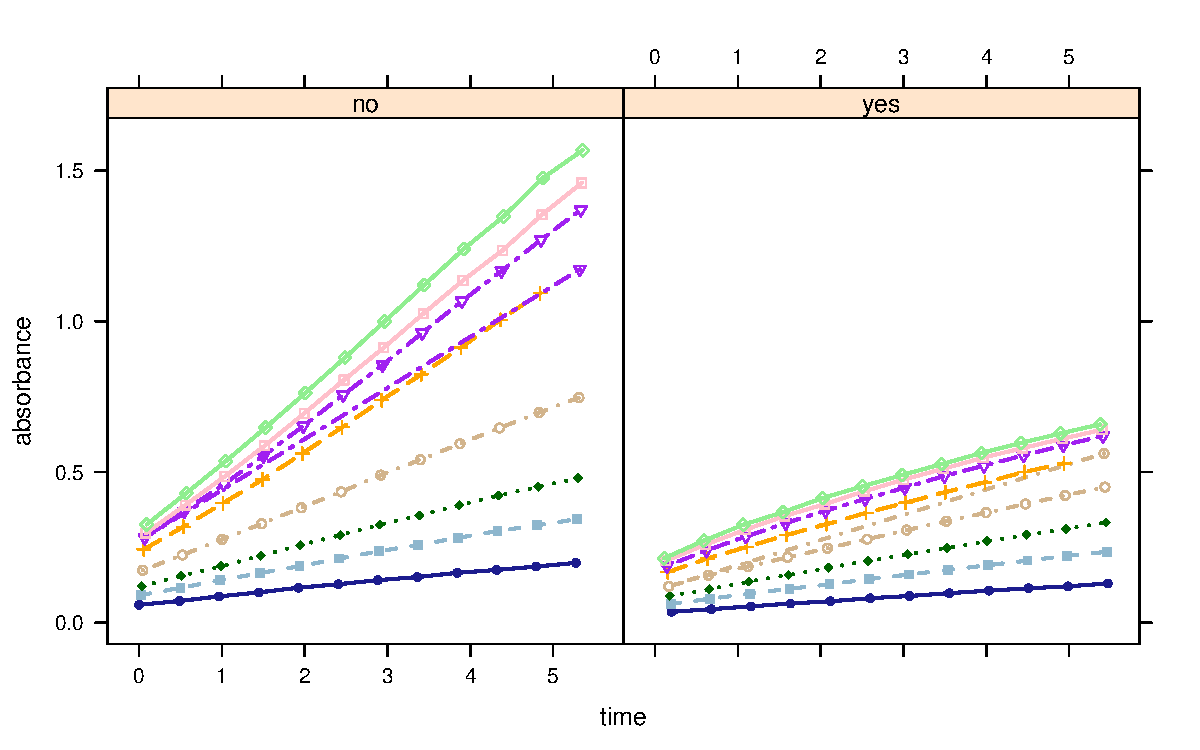
\includegraphics[width=.75\textwidth]{figures/modeling-unnamed-chunk-2} 

}


\end{knitrout}

\noindent
Not bad for student-collected data.

Now we need to estimate all those slopes.  We can do this all at once with a clever
choice of model.  For the following analysis, we'll use only the data without 
the inhibitor.
\begin{knitrout}
\definecolor{shadecolor}{rgb}{0.969, 0.969, 0.969}\color{fgcolor}\begin{kframe}
\begin{flushleft}
\ttfamily\noindent
\hlsymbol{mm}\hlkeyword{\usebox{\hlnormalsizeboxdollar}}\hlsymbol{S}{\ }\hlassignement{\usebox{\hlnormalsizeboxlessthan}-}{\ }\hlfunctioncall{factor}\hlkeyword{(}\hlsymbol{mm}\hlkeyword{\usebox{\hlnormalsizeboxdollar}}\hlsymbol{substrate}\hlkeyword{)}\hspace*{\fill}\\
\hlstd{}\hlsymbol{mmno}{\ }\hlassignement{\usebox{\hlnormalsizeboxlessthan}-}{\ }\hlfunctioncall{subset}\hlkeyword{(}\hlsymbol{mm}\hlkeyword{,}{\ }\hlsymbol{inhibitor}{\ }=={\ }\hlstring{"{}no"{}}\hlkeyword{)}\hspace*{\fill}\\
\hlstd{}\hlsymbol{slope.model}{\ }\hlassignement{\usebox{\hlnormalsizeboxlessthan}-}{\ }\hlfunctioncall{lm}\hlkeyword{(}\hlsymbol{absorbance}{\ }\hlkeyword{\urltilda{}}{\ }\hlsymbol{time}{\ }\hlkeyword{*}{\ }\hlsymbol{S}\hlkeyword{,}{\ }\hlargument{data}{\ }\hlargument{=}{\ }\hlsymbol{mmno}\hlkeyword{)}\hspace*{\fill}\\
\hlstd{}\hlfunctioncall{summary}\hlkeyword{(}\hlsymbol{slope.model}\hlkeyword{)}\mbox{}
\normalfont
\end{flushleft}
\begin{verbatim}

Call:
lm(formula = absorbance ~ time * S, data = mmno)

Residuals:
     Min       1Q   Median       3Q      Max 
-0.14643 -0.00300  0.00011  0.00270  0.04913 

Coefficients:
            Estimate Std. Error t value Pr(>|t|)
(Intercept)  0.06214    0.01075    5.78  1.4e-07
time         0.02641    0.00345    7.66  3.7e-11
S0.2         0.03173    0.01523    2.08  0.04041
S0.3         0.05935    0.01526    3.89  0.00021
S0.5         0.10578    0.01528    6.92  1.0e-09
S1           0.15577    0.01562    9.97  1.1e-15
S1.5         0.20656    0.01516   13.63  < 2e-16
S2           0.19780    0.01535   12.88  < 2e-16
S3           0.22729    0.01538   14.78  < 2e-16
time:S0.2    0.02179    0.00488    4.47  2.6e-05
time:S0.3    0.04235    0.00488    8.68  3.7e-13
time:S0.5    0.08312    0.00488   17.04  < 2e-16
time:S1      0.15245    0.00523   29.14  < 2e-16
time:S1.5    0.17090    0.00468   36.54  < 2e-16
time:S2      0.19665    0.00488   40.31  < 2e-16
time:S3      0.21396    0.00488   43.86  < 2e-16

Residual standard error: 0.0198 on 80 degrees of freedom
Multiple R-squared: 0.998,	Adjusted R-squared: 0.998 
F-statistic: 2.56e+03 on 15 and 80 DF,  p-value: <2e-16 

\end{verbatim}
\begin{flushleft}
\ttfamily\noindent
\hlfunctioncall{coef}\hlkeyword{(}\hlsymbol{slope.model}\hlkeyword{)}\mbox{}
\normalfont
\end{flushleft}
\begin{verbatim}
(Intercept)        time        S0.2        S0.3        S0.5          S1 
     0.0621      0.0264      0.0317      0.0594      0.1058      0.1558 
       S1.5          S2          S3   time:S0.2   time:S0.3   time:S0.5 
     0.2066      0.1978      0.2273      0.0218      0.0424      0.0831 
    time:S1   time:S1.5     time:S2     time:S3 
     0.1525      0.1709      0.1966      0.2140 
\end{verbatim}
\end{kframe}
\end{knitrout}


\begin{knitrout}
\definecolor{shadecolor}{rgb}{0.969, 0.969, 0.969}\color{fgcolor}\begin{kframe}
\begin{flushleft}
\ttfamily\noindent
\hlsymbol{mmSlopes}{\ }\hlassignement{\usebox{\hlnormalsizeboxlessthan}-}{\ }\hlfunctioncall{data.frame}\hlkeyword{(}\hlargument{S}{\ }\hlargument{=}{\ }\hlfunctioncall{as.numeric}\hlkeyword{(}\hlfunctioncall{levels}\hlkeyword{(}\hlsymbol{mmno}\hlkeyword{\usebox{\hlnormalsizeboxdollar}}\hlsymbol{S}\hlkeyword{)}\hlkeyword{)}\hlkeyword{,}{\ }\hlargument{v}{\ }\hlargument{=}{\ }\hlfunctioncall{coef}\hlkeyword{(}\hlsymbol{slope.model}\hlkeyword{)}\hlkeyword{[}\hlstring{"{}time"{}}\hlkeyword{]}{\ }\hlkeyword{+}\hspace*{\fill}\\
\hlstd{}{\ }{\ }{\ }{\ }\hlfunctioncall{c}\hlkeyword{(}\hlargument{\usebox{\hlnormalsizeboxbacktick}time:S0.1\usebox{\hlnormalsizeboxbacktick}}{\ }\hlargument{=}{\ }\hlnumber{0}\hlkeyword{,}{\ }\hlfunctioncall{coef}\hlkeyword{(}\hlsymbol{slope.model}\hlkeyword{)}\hlkeyword{[}\hlfunctioncall{paste}\hlkeyword{(}\hlstring{"{}time:S"{}}\hlkeyword{,}{\ }\hlfunctioncall{levels}\hlkeyword{(}\hlsymbol{mmno}\hlkeyword{\usebox{\hlnormalsizeboxdollar}}\hlsymbol{S}\hlkeyword{)}\hlkeyword{[}\hlkeyword{-}\hlnumber{1}\hlkeyword{]}\hlkeyword{,}\hspace*{\fill}\\
\hlstd{}{\ }{\ }{\ }{\ }{\ }{\ }{\ }{\ }\hlargument{sep}{\ }\hlargument{=}{\ }\hlstring{"{}"{}}\hlkeyword{)}\hlkeyword{]}\hlkeyword{)}\hlkeyword{)}\hspace*{\fill}\\
\hlstd{}\hlsymbol{mmSlopes}\mbox{}
\normalfont
\end{flushleft}
\begin{verbatim}
            S      v
time:S0.1 0.1 0.0264
time:S0.2 0.2 0.0482
time:S0.3 0.3 0.0688
time:S0.5 0.5 0.1095
time:S1   1.0 0.1789
time:S1.5 1.5 0.1973
time:S2   2.0 0.2231
time:S3   3.0 0.2404
\end{verbatim}
\end{kframe}
\end{knitrout}


\subsection{Fitting with Ordinary Least Squares}
Now we can fit our Michaelis-Menten model:
\begin{knitrout}
\definecolor{shadecolor}{rgb}{0.969, 0.969, 0.969}\color{fgcolor}\begin{kframe}
\begin{flushleft}
\ttfamily\noindent
\hlsymbol{mmModel}{\ }\hlassignement{\usebox{\hlnormalsizeboxlessthan}-}{\ }\hlfunctioncall{lm}\hlkeyword{(}\hlkeyword{(}\hlnumber{1}\hlkeyword{/}\hlsymbol{v}\hlkeyword{)}{\ }\hlkeyword{\urltilda{}}{\ }\hlfunctioncall{I}\hlkeyword{(}\hlnumber{1}\hlkeyword{/}\hlsymbol{S}\hlkeyword{)}\hlkeyword{,}{\ }\hlsymbol{mmSlopes}\hlkeyword{)}\hspace*{\fill}\\
\hlstd{}\hlfunctioncall{summary}\hlkeyword{(}\hlsymbol{mmModel}\hlkeyword{)}\mbox{}
\normalfont
\end{flushleft}
\begin{verbatim}

Call:
lm(formula = (1/v) ~ I(1/S), data = mmSlopes)

Residuals:
   Min     1Q Median     3Q    Max 
-0.544 -0.239  0.119  0.209  0.449 

Coefficients:
            Estimate Std. Error t value Pr(>|t|)
(Intercept)   2.5915     0.1973    13.1  1.2e-05
I(1/S)        3.5408     0.0468    75.6  3.6e-10

Residual standard error: 0.41 on 6 degrees of freedom
Multiple R-squared: 0.999,	Adjusted R-squared: 0.999 
F-statistic: 5.72e+03 on 1 and 6 DF,  p-value: 3.61e-10 

\end{verbatim}
\begin{flushleft}
\ttfamily\noindent
\hlsymbol{alpha.hat}{\ }\hlassignement{\usebox{\hlnormalsizeboxlessthan}-}{\ }\hlnumber{1}\hlkeyword{/}\hlfunctioncall{coef}\hlkeyword{(}\hlsymbol{mmModel}\hlkeyword{)}\hlkeyword{[}\hlnumber{1}\hlkeyword{]}\hspace*{\fill}\\
\hlstd{}\hlsymbol{beta.hat}{\ }\hlassignement{\usebox{\hlnormalsizeboxlessthan}-}{\ }\hlfunctioncall{coef}\hlkeyword{(}\hlsymbol{mmModel}\hlkeyword{)}\hlkeyword{[}\hlnumber{2}\hlkeyword{]}{\ }\hlkeyword{*}{\ }\hlsymbol{alpha.hat}\hspace*{\fill}\\
\hlstd{}\hlfunctioncall{c}\hlkeyword{(}\hlargument{alpha.hat}{\ }\hlargument{=}{\ }\hlsymbol{alpha.hat}\hlkeyword{,}{\ }\hlargument{beta.hat}{\ }\hlargument{=}{\ }\hlsymbol{beta.hat}\hlkeyword{)}\mbox{}
\normalfont
\end{flushleft}
\begin{verbatim}
alpha.hat.(Intercept)       beta.hat.I(1/S) 
                0.386                 1.366 
\end{verbatim}
\begin{flushleft}
\ttfamily\noindent
\hlsymbol{f}{\ }\hlassignement{\usebox{\hlnormalsizeboxlessthan}-}{\ }\hlfunctioncall{makeFun}\hlkeyword{(}\hlsymbol{mmModel}\hlkeyword{)}\hspace*{\fill}\\
\hlstd{}\hlfunctioncall{xyplot}\hlkeyword{(}\hlnumber{1}\hlkeyword{/}\hlsymbol{v}{\ }\hlkeyword{\urltilda{}}{\ }\hlnumber{1}\hlkeyword{/}\hlsymbol{S}\hlkeyword{,}{\ }\hlsymbol{mmSlopes}\hlkeyword{,}{\ }\hlargument{main}{\ }\hlargument{=}{\ }\hlstring{"{}1/v{\ }vs.{\ }1/S{\ }(as{\ }fit)"{}}\hlkeyword{)}\hspace*{\fill}\\
\hlstd{}\hlsymbol{g}{\ }\hlassignement{\usebox{\hlnormalsizeboxlessthan}-}{\ }\hlfunctioncall{makeFun}\hlkeyword{(}\hlfunctioncall{f}\hlkeyword{(}\hlnumber{1}\hlkeyword{/}\hlsymbol{x}\hlkeyword{)}{\ }\hlkeyword{\urltilda{}}{\ }\hlsymbol{x}\hlkeyword{)}\hspace*{\fill}\\
\hlstd{}\hlfunctioncall{plotFun}\hlkeyword{(}\hlfunctioncall{g}\hlkeyword{(}\hlsymbol{x}\hlkeyword{)}{\ }\hlkeyword{\urltilda{}}{\ }\hlsymbol{x}\hlkeyword{,}{\ }\hlargument{add}{\ }\hlargument{=}{\ }\hlnumber{TRUE}\hlkeyword{,}{\ }\hlargument{col}{\ }\hlargument{=}{\ }\hlstring{"{}navy"{}}\hlkeyword{,}{\ }\hlargument{alpha}{\ }\hlargument{=}{\ }\hlnumber{0.4}\hlkeyword{)}\hspace*{\fill}\\
\hlstd{}\hlfunctioncall{xyplot}\hlkeyword{(}\hlsymbol{v}{\ }\hlkeyword{\urltilda{}}{\ }\hlsymbol{S}\hlkeyword{,}{\ }\hlsymbol{mmSlopes}\hlkeyword{,}{\ }\hlargument{ylim}{\ }\hlargument{=}{\ }\hlfunctioncall{c}\hlkeyword{(}\hlnumber{0}\hlkeyword{,}{\ }\hlnumber{0.3}\hlkeyword{)}\hlkeyword{,}{\ }\hlargument{main}{\ }\hlargument{=}{\ }\hlstring{"{}v{\ }vs.{\ }S{\ }(as{\ }desired)"{}}\hlkeyword{)}\hspace*{\fill}\\
\hlstd{}\hlfunctioncall{plotFun}\hlkeyword{(}\hlnumber{1}\hlkeyword{/}\hlfunctioncall{f}\hlkeyword{(}\hlsymbol{S}\hlkeyword{)}{\ }\hlkeyword{\urltilda{}}{\ }\hlsymbol{S}\hlkeyword{,}{\ }\hlargument{add}{\ }\hlargument{=}{\ }\hlnumber{TRUE}\hlkeyword{,}{\ }\hlargument{col}{\ }\hlargument{=}{\ }\hlstring{"{}navy"{}}\hlkeyword{,}{\ }\hlargument{alpha}{\ }\hlargument{=}{\ }\hlnumber{0.4}\hlkeyword{)}\mbox{}
\normalfont
\end{flushleft}
\end{kframe}

{\centering 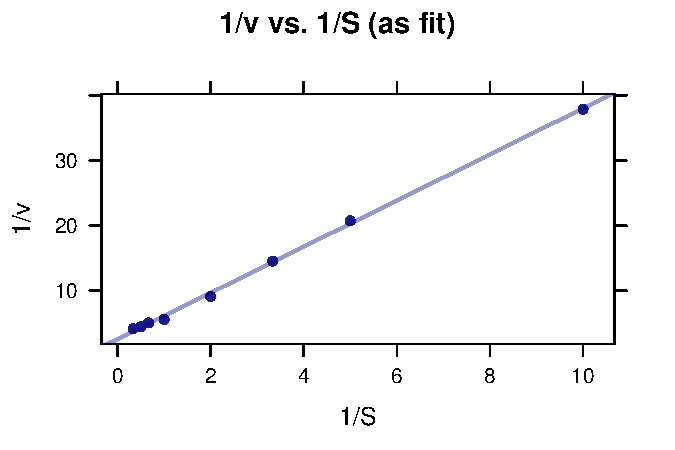
\includegraphics[width=.47\textwidth]{figures/modeling-mmModel1} 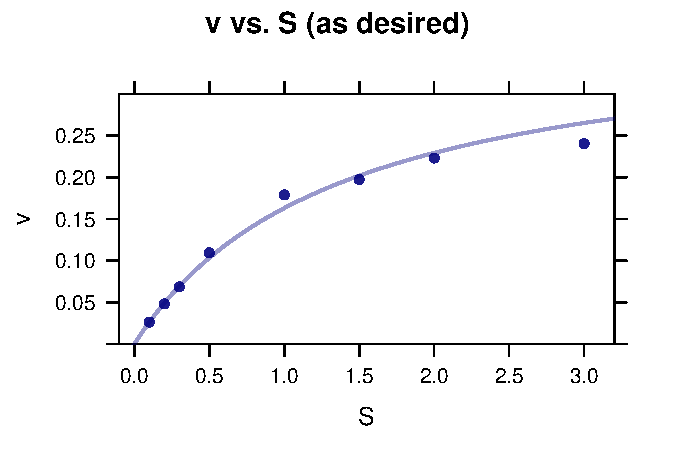
\includegraphics[width=.47\textwidth]{figures/modeling-mmModel2} 

}


\end{knitrout}


Doing this we see some issues.  Although there is a nice tight fit of the transformed 
data to the least squares regression line, the fit doesn't look nearly as good after 
back-transforming to the original scales.  In particular, errors are much larger for larger
values of $S$.  Or thought about the other way around, the way we have fit the model 
has forced the fit to be extremely good for small values of $S$ at the cost of allowing
much poorer fits for larger values of $S$.  This is becuase the transformations
transform the scale for the residuals as well as for the inputs.  Note too that the distribution of values of $1/S$ is not nearly as uniform as it is for $S$.

\subsection{Fitting with Nonlinear Least Squares}
We can do better if we use nonlinear least squares instead of tranforming and using least
squares.  In non-linear least squares we fit a parameterized function of arbitrary form
by determining (well, estimating anyway) the values of the parameters that 
minimize the sum of the squares of the residuals
\[
SS(\alpha, \beta) = \sum_{i=1}^n ( v_i - f(\alpha, \beta; S_i) )^2
\]
This approach will be less forgiving of such large residuals for large values of $S$.
We lose something in the exchange, however.  It is not longer the case that simple
closed-form formulas exist for the estimates.  This means that we will need to rely
on numerical estimation.  
Furthermore the estimators are not guaranteed to be
unbiased.

\begin{knitrout}
\definecolor{shadecolor}{rgb}{0.969, 0.969, 0.969}\color{fgcolor}\begin{kframe}
\begin{flushleft}
\ttfamily\noindent
\hlcomment{\usebox{\hlnormalsizeboxhash}{\ }we{\ }provide{\ }nls(){\ }with{\ }our{\ }estimates{\ }from{\ }above{\ }as{\ }a{\ }starting{\ }point.}\hspace*{\fill}\\
\hlstd{}\hlsymbol{model.nls}{\ }\hlassignement{\usebox{\hlnormalsizeboxlessthan}-}{\ }\hlfunctioncall{nls}\hlkeyword{(}\hlsymbol{v}{\ }\hlkeyword{\urltilda{}}{\ }\hlsymbol{alpha}{\ }\hlkeyword{*}{\ }\hlsymbol{S}\hlkeyword{/}\hlkeyword{(}\hlsymbol{beta}{\ }\hlkeyword{+}{\ }\hlsymbol{S}\hlkeyword{)}\hlkeyword{,}{\ }\hlargument{data}{\ }\hlargument{=}{\ }\hlsymbol{mmSlopes}\hlkeyword{,}{\ }\hlargument{start}{\ }\hlargument{=}{\ }\hlfunctioncall{list}\hlkeyword{(}\hlargument{alpha}{\ }\hlargument{=}{\ }\hlsymbol{alpha.hat}\hlkeyword{,}\hspace*{\fill}\\
\hlstd{}{\ }{\ }{\ }{\ }\hlargument{beta}{\ }\hlargument{=}{\ }\hlsymbol{beta.hat}\hlkeyword{)}\hlkeyword{)}\hspace*{\fill}\\
\hlstd{}\hlfunctioncall{summary}\hlkeyword{(}\hlsymbol{model.nls}\hlkeyword{)}\mbox{}
\normalfont
\end{flushleft}
\begin{verbatim}

Formula: v ~ alpha * S/(beta + S)

Parameters:
      Estimate Std. Error t value Pr(>|t|)
alpha   0.3297     0.0163   20.24  9.4e-07
beta    0.9979     0.1191    8.38  0.00016

Residual standard error: 0.00782 on 6 degrees of freedom

Number of iterations to convergence: 5 
Achieved convergence tolerance: 6.84e-06 

\end{verbatim}
\begin{flushleft}
\ttfamily\noindent
\hlfunctioncall{xyplot}\hlkeyword{(}\hlsymbol{v}{\ }\hlkeyword{\urltilda{}}{\ }\hlsymbol{S}\hlkeyword{,}{\ }\hlsymbol{mmSlopes}\hlkeyword{,}{\ }\hlargument{ylim}{\ }\hlargument{=}{\ }\hlfunctioncall{c}\hlkeyword{(}\hlnumber{0}\hlkeyword{,}{\ }\hlnumber{0.35}\hlkeyword{)}\hlkeyword{)}\hspace*{\fill}\\
\hlstd{}\hlfunctioncall{ladd}\hlkeyword{(}\hlfunctioncall{panel.xyplot}\hlkeyword{(}\hlsymbol{mmSlopes}\hlkeyword{\usebox{\hlnormalsizeboxdollar}}\hlsymbol{S}\hlkeyword{,}{\ }\hlfunctioncall{predict}\hlkeyword{(}\hlsymbol{model.nls}\hlkeyword{)}\hlkeyword{,}{\ }\hlargument{type}{\ }\hlargument{=}{\ }\hlstring{"{}l"{}}\hlkeyword{,}{\ }\hlargument{col}{\ }\hlargument{=}{\ }\hlstring{"{}navy"{}}\hlkeyword{,}\hspace*{\fill}\\
\hlstd{}{\ }{\ }{\ }{\ }\hlargument{alpha}{\ }\hlargument{=}{\ }\hlnumber{0.4}\hlkeyword{)}\hlkeyword{)}\mbox{}
\normalfont
\end{flushleft}
\end{kframe}

{\centering 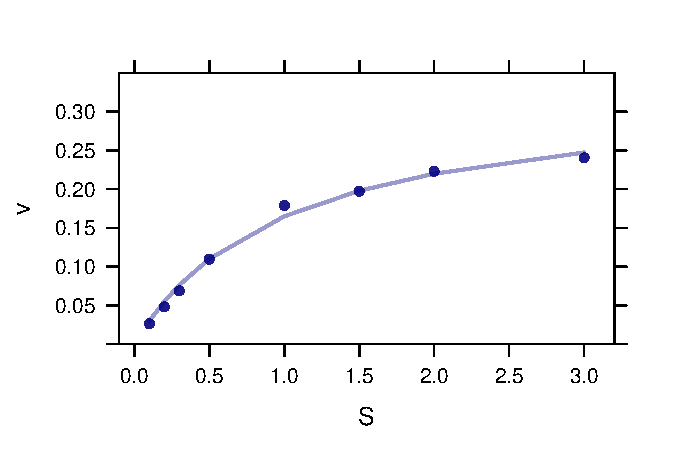
\includegraphics[width=.47\textwidth]{figures/modeling-nls} 

}


\end{knitrout}

As expected, the fit is much better for larger values of $S$ and we've lost very little for smaller values of $S$.

Now that we have (two sets of) estimates for $\alpha$ and $\beta$, we should
pause a moment to see what these parameters tell us about the chemistry.
Recall Equation (\ref{eq:MichMent})
	\begin{align*}
	v = \frac{ \alpha [S] }{ \beta + [S] }
	\end{align*}
As $[S]$ increases,
\[
	\frac{ \alpha [S] }{ \beta + [S] } \nearrow \alpha
\]
so $\alpha$ gives the horizontal asymptote representing the maximum velocity.
And if $[S] = \beta$, we get
\[
v = \frac{ \alpha [S] }{ [S] + [S] } = \frac{\alpha}{2} \; ,
\]
so $\beta$ is the value of $[S]$ that gives half the maximum velocity.

\begin{knitrout}
\definecolor{shadecolor}{rgb}{0.969, 0.969, 0.969}\color{fgcolor}\begin{kframe}
\begin{flushleft}
\ttfamily\noindent
\hlfunctioncall{xyplot}\hlkeyword{(}\hlsymbol{v}{\ }\hlkeyword{\urltilda{}}{\ }\hlsymbol{S}\hlkeyword{,}{\ }\hlsymbol{mmSlopes}\hlkeyword{,}{\ }\hlargument{ylim}{\ }\hlargument{=}{\ }\hlfunctioncall{c}\hlkeyword{(}\hlnumber{0}\hlkeyword{,}{\ }\hlnumber{1.1}{\ }\hlkeyword{*}{\ }\hlsymbol{alpha.hat}\hlkeyword{)}\hlkeyword{,}{\ }\hlargument{main}{\ }\hlargument{=}{\ }\hlstring{"{}linear{\ }least{\ }squares{\ }fit"{}}\hlkeyword{)}\hspace*{\fill}\\
\hlstd{}\hlfunctioncall{plotFun}\hlkeyword{(}\hlnumber{1}\hlkeyword{/}\hlfunctioncall{f}\hlkeyword{(}\hlsymbol{S}\hlkeyword{)}{\ }\hlkeyword{\urltilda{}}{\ }\hlsymbol{S}\hlkeyword{,}{\ }\hlargument{add}{\ }\hlargument{=}{\ }\hlnumber{TRUE}\hlkeyword{,}{\ }\hlargument{col}{\ }\hlargument{=}{\ }\hlstring{"{}navy"{}}\hlkeyword{,}{\ }\hlargument{alpha}{\ }\hlargument{=}{\ }\hlnumber{0.4}\hlkeyword{)}\hspace*{\fill}\\
\hlstd{}\hlfunctioncall{ladd}\hlkeyword{(}\hlfunctioncall{panel.abline}\hlkeyword{(}\hlargument{h}{\ }\hlargument{=}{\ }\hlsymbol{alpha.hat}\hlkeyword{,}{\ }\hlargument{col}{\ }\hlargument{=}{\ }\hlstring{"{}red"{}}\hlkeyword{,}{\ }\hlargument{alpha}{\ }\hlargument{=}{\ }\hlnumber{0.4}\hlkeyword{)}\hlkeyword{)}\hspace*{\fill}\\
\hlstd{}\hlfunctioncall{ladd}\hlkeyword{(}\hlfunctioncall{panel.abline}\hlkeyword{(}\hlargument{v}{\ }\hlargument{=}{\ }\hlsymbol{beta.hat}\hlkeyword{,}{\ }\hlargument{col}{\ }\hlargument{=}{\ }\hlstring{"{}darkgreen"{}}\hlkeyword{,}{\ }\hlargument{alpha}{\ }\hlargument{=}{\ }\hlnumber{0.4}\hlkeyword{)}\hlkeyword{)}\hspace*{\fill}\\
\hlstd{}\hlfunctioncall{xyplot}\hlkeyword{(}\hlsymbol{v}{\ }\hlkeyword{\urltilda{}}{\ }\hlsymbol{S}\hlkeyword{,}{\ }\hlsymbol{mmSlopes}\hlkeyword{,}{\ }\hlargument{ylim}{\ }\hlargument{=}{\ }\hlfunctioncall{c}\hlkeyword{(}\hlnumber{0}\hlkeyword{,}{\ }\hlnumber{1.1}{\ }\hlkeyword{*}{\ }\hlsymbol{alpha.hat}\hlkeyword{)}\hlkeyword{,}{\ }\hlargument{main}{\ }\hlargument{=}{\ }\hlstring{"{}non-linear{\ }least{\ }squares{\ }fit"{}}\hlkeyword{)}\hspace*{\fill}\\
\hlstd{}\hlfunctioncall{ladd}\hlkeyword{(}\hlfunctioncall{panel.xyplot}\hlkeyword{(}\hlsymbol{mmSlopes}\hlkeyword{\usebox{\hlnormalsizeboxdollar}}\hlsymbol{S}\hlkeyword{,}{\ }\hlfunctioncall{predict}\hlkeyword{(}\hlsymbol{model.nls}\hlkeyword{)}\hlkeyword{,}{\ }\hlargument{type}{\ }\hlargument{=}{\ }\hlstring{"{}l"{}}\hlkeyword{,}{\ }\hlargument{col}{\ }\hlargument{=}{\ }\hlstring{"{}navy"{}}\hlkeyword{,}\hspace*{\fill}\\
\hlstd{}{\ }{\ }{\ }{\ }\hlargument{alpha}{\ }\hlargument{=}{\ }\hlnumber{0.4}\hlkeyword{)}\hlkeyword{)}\hspace*{\fill}\\
\hlstd{}\hlfunctioncall{ladd}\hlkeyword{(}\hlfunctioncall{panel.abline}\hlkeyword{(}\hlargument{h}{\ }\hlargument{=}{\ }\hlfunctioncall{coef}\hlkeyword{(}\hlsymbol{model.nls}\hlkeyword{)}\hlkeyword{[}\hlnumber{1}\hlkeyword{]}\hlkeyword{,}{\ }\hlargument{col}{\ }\hlargument{=}{\ }\hlstring{"{}red"{}}\hlkeyword{,}{\ }\hlargument{alpha}{\ }\hlargument{=}{\ }\hlnumber{0.4}\hlkeyword{)}\hlkeyword{)}\hspace*{\fill}\\
\hlstd{}\hlfunctioncall{ladd}\hlkeyword{(}\hlfunctioncall{panel.abline}\hlkeyword{(}\hlargument{v}{\ }\hlargument{=}{\ }\hlfunctioncall{coef}\hlkeyword{(}\hlsymbol{model.nls}\hlkeyword{)}\hlkeyword{[}\hlnumber{2}\hlkeyword{]}\hlkeyword{,}{\ }\hlargument{col}{\ }\hlargument{=}{\ }\hlstring{"{}darkgreen"{}}\hlkeyword{,}{\ }\hlargument{alpha}{\ }\hlargument{=}{\ }\hlnumber{0.4}\hlkeyword{)}\hlkeyword{)}\mbox{}
\normalfont
\end{flushleft}
\end{kframe}

{\centering 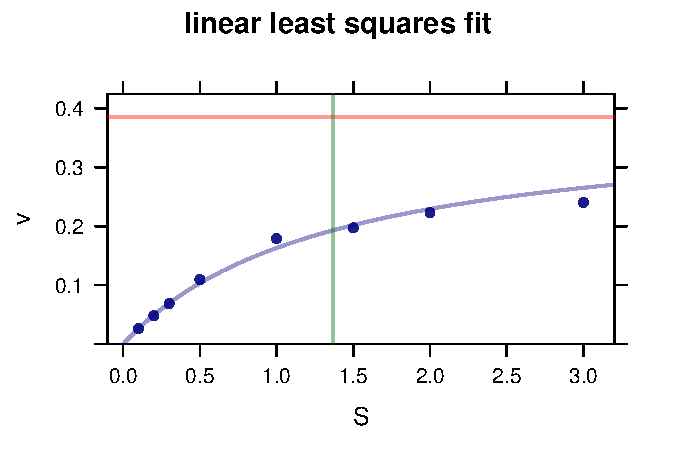
\includegraphics[width=.47\textwidth]{figures/modeling-unnamed-chunk-31} 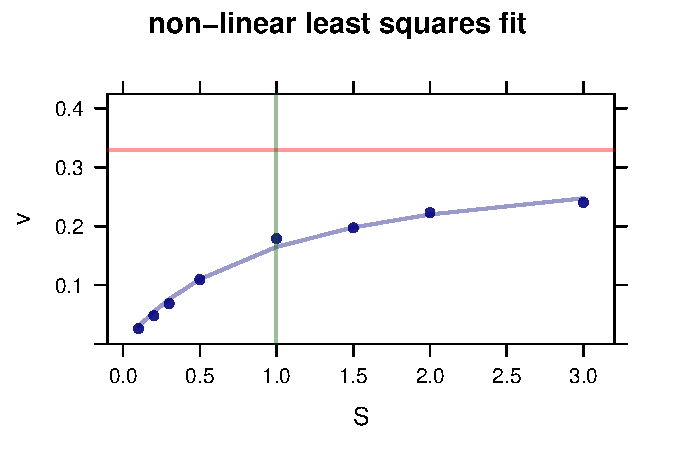
\includegraphics[width=.47\textwidth]{figures/modeling-unnamed-chunk-32} 

}


\end{knitrout}



\end{document}
